\documentclass{pl-slide}

\usepackage[british]{babel}
\usepackage[british]{datetime2}

%Information to be included in the title page:
\title{DHT Routing Table Health}
\subtitle{Our DHT is in good shape!}
\author{Guillaume Michel}
\handle{@guissou}
\group{ProbeLab}
\institute{Protocol Labs}
%\event{IPFS þing}
%\date{\DTMdate{2022-07-15}}
\event{The Mother of ALL DEMO DAYS}
\date{\DTMdate{2022-07-07}}

\begin{document}


\frame{\titlepage}

\begin{frame}
\frametitle{Kademlia DHT Routing Table}
\begin{itemize}
	\item A Distributed Hash Table (DHT) is a decentralized overlay network
	\item Each node has to know some other peers to be connected to the network, this set of peers is the node's Routing Table
	\item Kademlia keeps peers in \texttt{k-buckets} sorting the \texttt{peer\_id} by XOR distance (or Common Prefix Length). Each bucket is capped at 20 peers
\end{itemize}
\end{frame}

\begin{frame}
\frametitle{Example: Routing Table of peer \texttt{01101000}}
\begin{columns}[onlytextwidth,t]
\begin{column}{0.19\textwidth}
	\textbf{Bucket 0}
   	\begin{enumerate}
   		\item 11010111
   		\item 10001011
   		\item 10101110
   		\item 11110101
   		\item 10000010
   		\item 11010100
   		\item 11000100
   		\item ...
   	\end{enumerate}
\end{column}
\begin{column}{0.19\textwidth}
	\textbf{Bucket 1}
   \begin{enumerate}
   		\item \textbf{0}0110101
   		\item \textbf{0}0001000
   		\item \textbf{0}0111011
   		\item \textbf{0}0101101
   		\item \textbf{0}0110100
   \end{enumerate}
\end{column}
\begin{column}{0.19\textwidth}
	\textbf{Bucket 2}
   \begin{enumerate}
   		\item \textbf{01}011101
   		\item \textbf{01}001111
   		\item \textbf{01}010110
   \end{enumerate}
\end{column}
\begin{column}{0.19\textwidth}
	\textbf{Bucket 3}
   \begin{enumerate}
   		\item \textbf{011}11011
   		\item \textbf{011}10001
   \end{enumerate}
\end{column}
\begin{column}{0.19\textwidth}
	\textbf{Bucket 4}
   	\begin{enumerate}
   		\item \textbf{0110}0011
   \end{enumerate}
\end{column}
\end{columns}
\end{frame}

\iffalse
\begin{frame}
\frametitle{\texttt{k-bucket} replacement policy}
\begin{itemize}
    \item \texttt{Kademlia}: only when a bucket is full and there is a new candidate, least-recently seen and unreachable node gets evicted, but live nodes are never evicted
	\bigskip    
    \item \texttt{kubo} implementation: periodically ping nodes that it didn't hear of recently, and evict them if they don't respond
\end{itemize}
\end{frame}
\fi

\begin{frame}
\frametitle{Measurements data}
\begin{itemize}
    \item The Nebula Crawler crawls the IPFS network and provides all peers in the network along with their routing table for a point in time
    \item Data taken from 28 crawls over 1 week (4 crawls per day) starting on \texttt{2022-04-19}
\end{itemize}
\end{frame}

\begin{frame}
\frametitle{Methodology}
\begin{itemize}
	\item The Nebula Crawler provides a global snapshot of the network
	\item We can reconstruct the \texttt{k-buckets} of all peers by computing the XOR distance between a \texttt{peer\_id} and the \texttt{peer\_id}s of all peers in its routing table
	\item From the global snapshot we can find the closest peers to every other peer and verify if any peer is missing from a \texttt{k-bucket}
    \item Caveat: XOR distance is non-linear! Computationnaly expensive to find the closest peers to a specific \texttt{peer\_id}. A python Binary Trie implementation was built for this purpose
\end{itemize}
\end{frame}


\begin{frame}
\frametitle{Unreachable peers in the Routing Table}

\begin{columns}[onlytextwidth]
\begin{column}{0.38\textwidth}
Unreachable peers may still be referenced in other peers routing tables (stale entries)
\bigskip
   \begin{itemize}
   		\item Average for buckets \texttt{0} to \texttt{8}: \texttt{3.8\%} $\sim$ \texttt{0.75} peers
   		\item Average for buckets \texttt{9} to \texttt{21}: \texttt{15\%}
   \end{itemize}
\end{column}
\begin{column}{0.58\textwidth}
    \begin{center}
		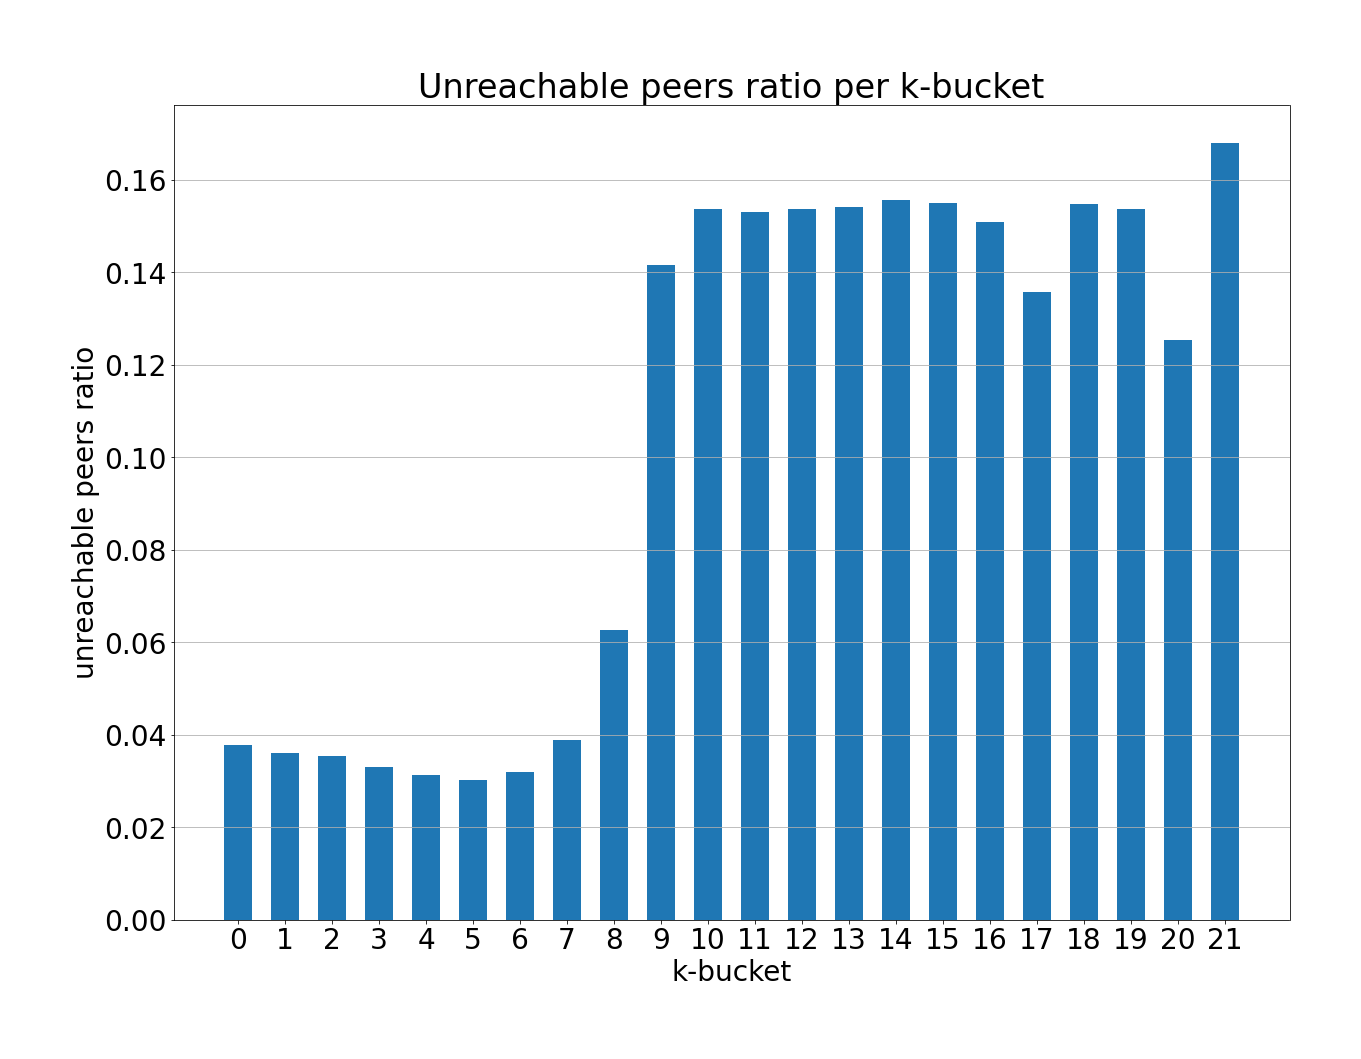
\includegraphics[width=\textwidth]{plots/unreachable-peers.png}
    \end{center}
\end{column}
\end{columns}
\end{frame}

\begin{frame}
\frametitle{Peers distribution in the k-buckets}

\begin{columns}[onlytextwidth]
\begin{column}{0.38\textwidth}
   	\begin{itemize}
   		\item Peers distribution in bucket follows an exponential growth, capped at 20
   		\item Buckets \texttt{0-8} are missing on average \texttt{0.12} peers per bucket
   		\item Buckets \texttt{9-14} are missing on average \texttt{0.53} peers per bucket
   	\end{itemize}
\end{column}
\begin{column}{0.58\textwidth}
    \begin{center}
		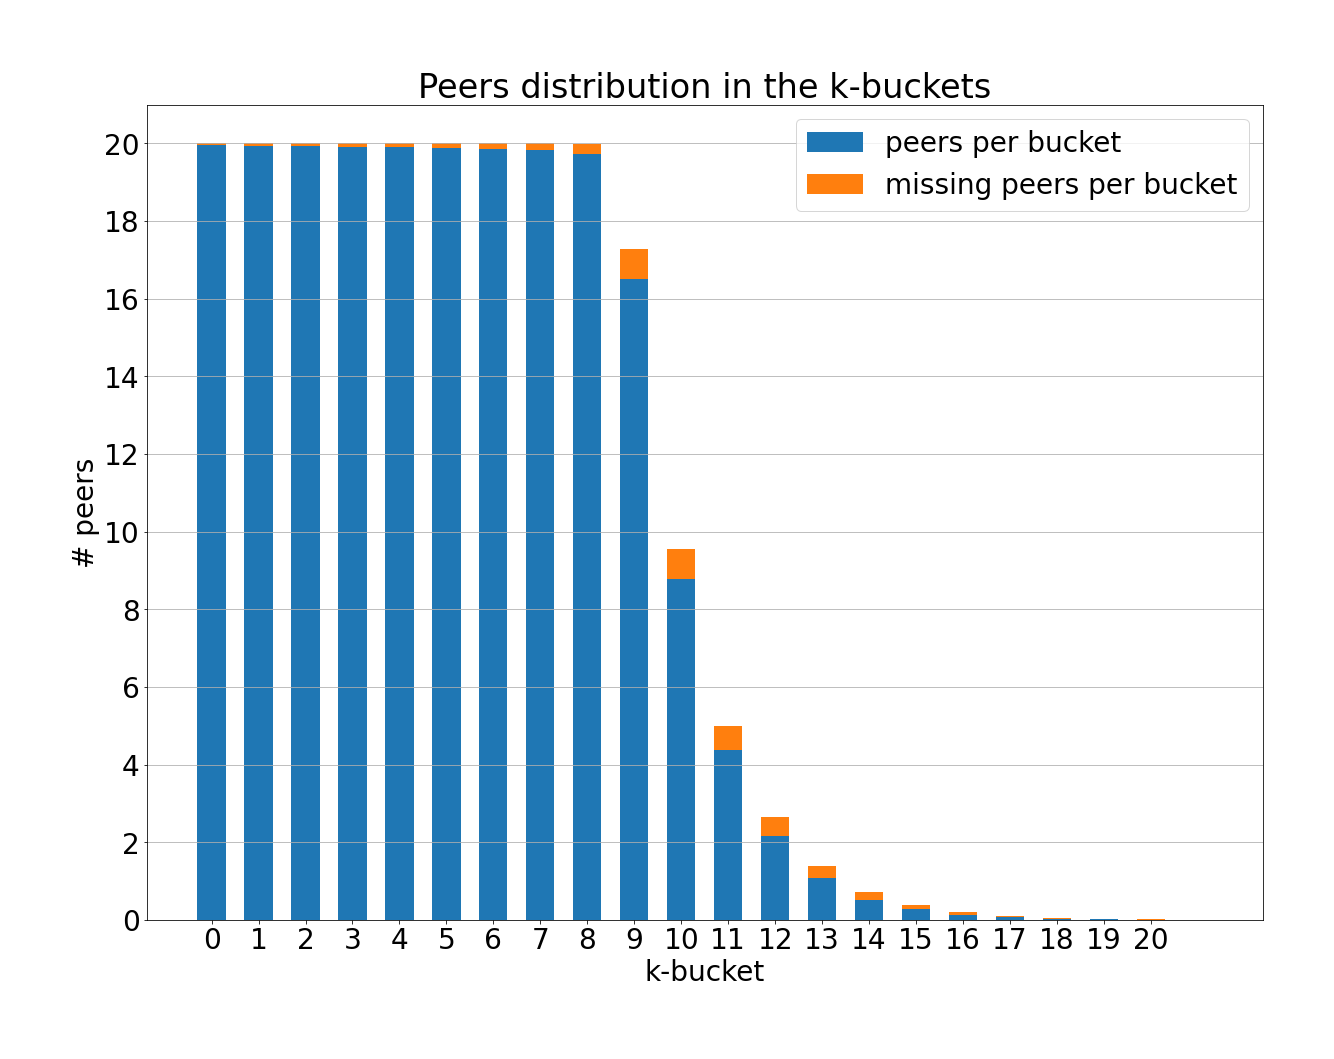
\includegraphics[width=\textwidth]{plots/peers-distribution-including-missing.png}
    \end{center}
\end{column}
\end{columns}
\end{frame}


\begin{frame}
\frametitle{20 closest peers awareness}

\begin{columns}[onlytextwidth]
\begin{column}{0.38\textwidth}
\begin{enumerate}
   	\item Probability Density Function (PDF)
   	\item Cumulative Distribution Function (CDF)
\end{enumerate}
\bigskip
\begin{itemize}
   	\item \texttt{61.1\%} of the peers know all their 20 closest peers
   	\item \texttt{95.2\%} of the peers know at least 18 of their 20 closest peers
\end{itemize}
\end{column}
\begin{column}{0.58\textwidth}
    \begin{center}
		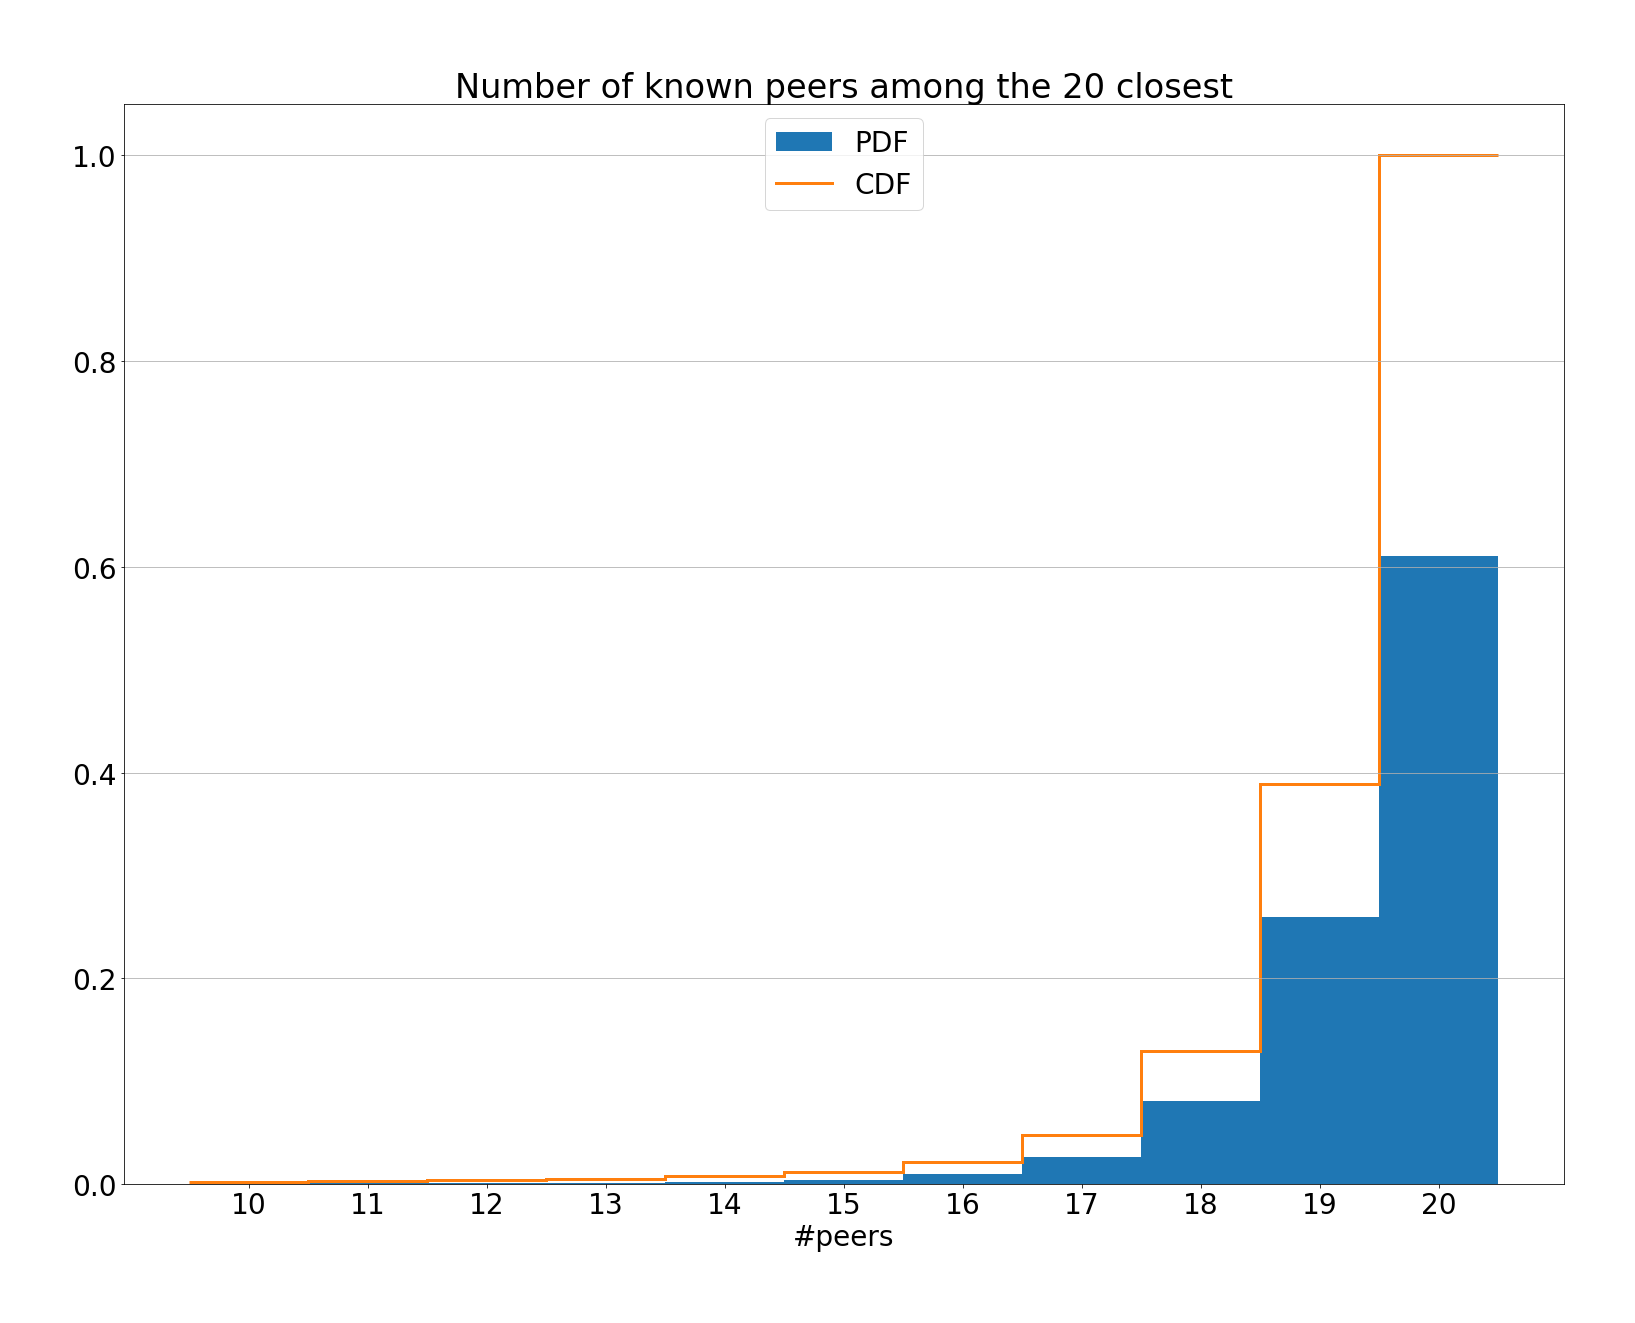
\includegraphics[width=\textwidth]{plots/known-peers-among-20-closest.png}
    \end{center}
\end{column}
\end{columns}
\end{frame}

\iffalse

\begin{frame}
\frametitle{Diversity in the k-buckets}

\begin{itemize}
	\item Live peers never get replaced in the \texttt{k-buckets} by design
	\item Eventually, buckets with many candidates (e.g buckets \texttt{0-1}) will be filled almost exclusively with a small number of very stable peers
	\item Routing for content \textit{far away} (in XOR distance) may become centralized on a small set of peers
	\item Bad for decentralization :(
\end{itemize}
\end{frame}

\begin{frame}
\frametitle{New measurements}
\begin{columns}[onlytextwidth]
\begin{column}{0.38\textwidth}
   \begin{itemize}
   		\item Measurements for 10 consecutive weeks starting on \texttt{2022-02-16}
   		\item Each week's measurements are based on data from 14 crawls (2x/day)
   		\item Diversity in \texttt{k-buckets} is measured as the number of distinct \texttt{peer\_id}s observed in each bucket for all peers
   \end{itemize}
\end{column}
\begin{column}{0.58\textwidth}
    \begin{center}
		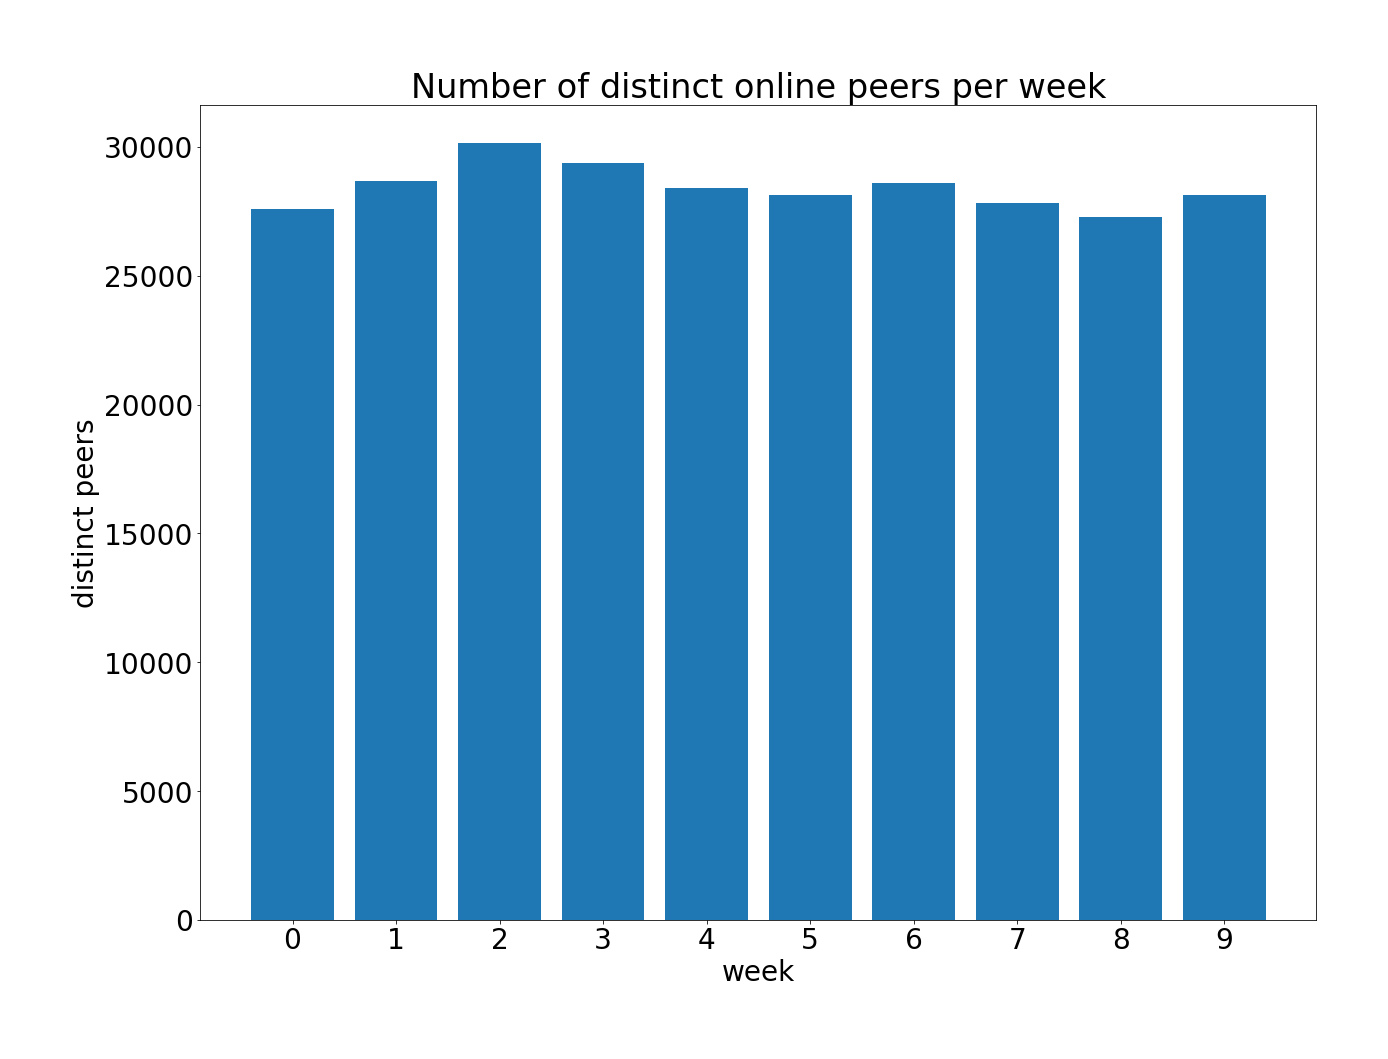
\includegraphics[width=\textwidth]{plots/online-peers-per-week.png}
    \end{center}
\end{column}
\end{columns}
\end{frame}

\begin{frame}
\frametitle{Diversity in each k-buckets}

\begin{columns}[onlytextwidth]
\begin{column}{0.38\textwidth}
   \begin{itemize}
   		\item Buckets \texttt{10+}: non-full buckets $\rightarrow$ low diversity
   		\item Bucket \texttt{9}: bucket just full \\$\rightarrow$ highest diversity
   		\item Buckets \texttt{0-1}: many candidates, only the most stable don't get evicted \\$\rightarrow$ lower diversity
   		\item We expect diversity in buckets \texttt{0-1} to decrease over time
   \end{itemize}
\end{column}
\begin{column}{0.58\textwidth}
    \begin{center}
		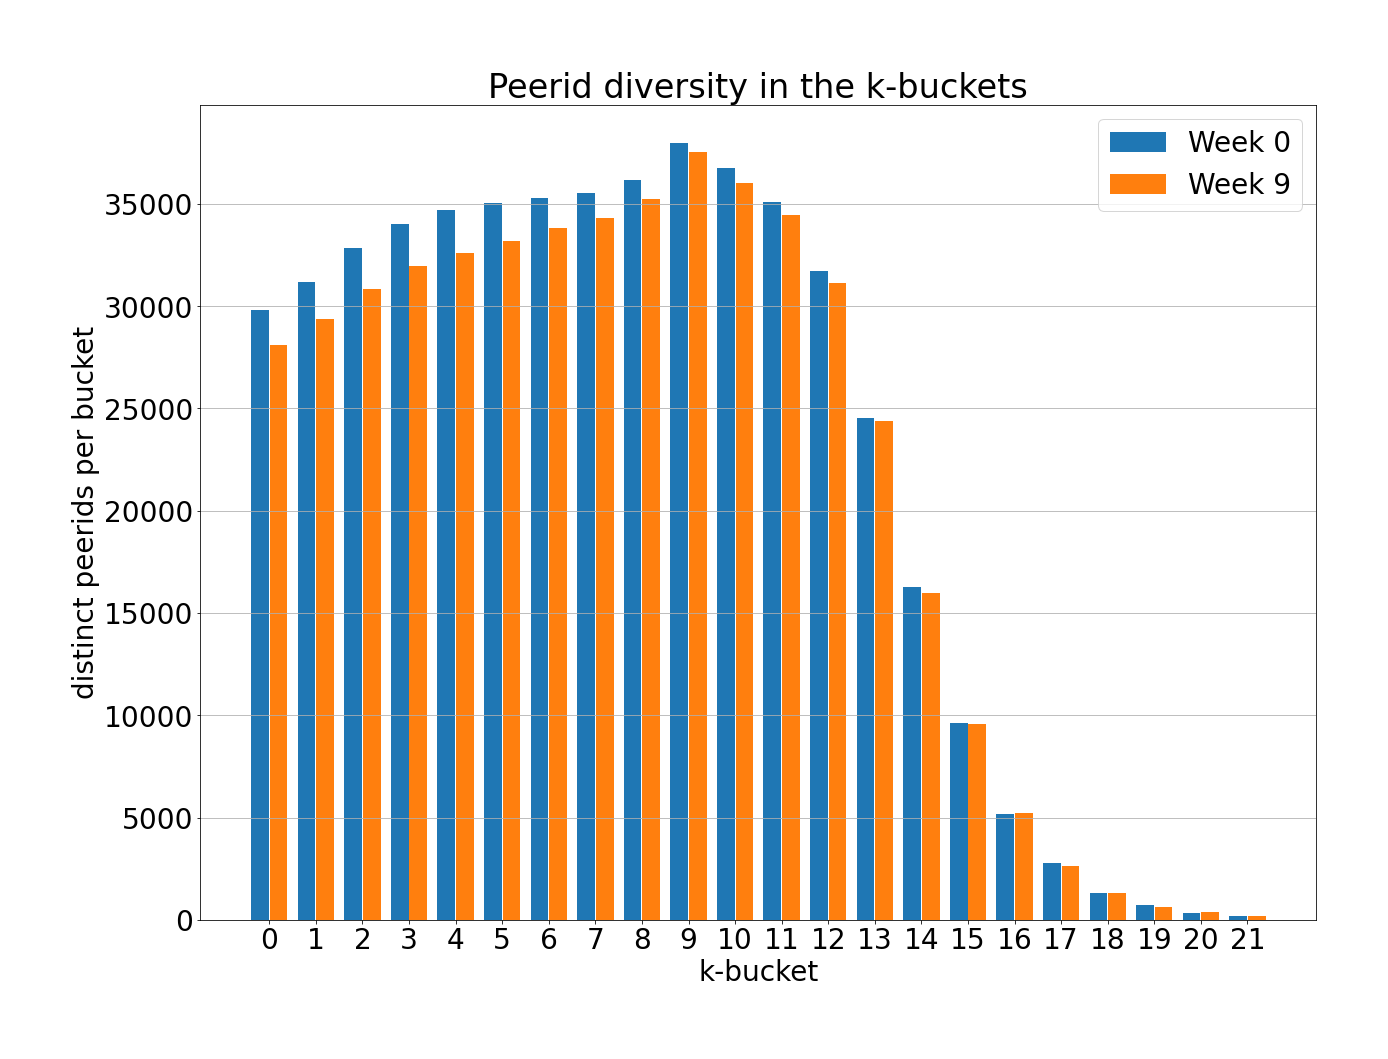
\includegraphics[width=\textwidth]{plots/diversity-in-buckets.png}
    \end{center}
\end{column}
\end{columns}
\end{frame}

\begin{frame}
\frametitle{Diversity evolution over time}

\begin{columns}[onlytextwidth]
\begin{column}{0.38\textwidth}
   Moving average difference between week 1 and week 8:
   \begin{itemize}
   		\item[] Bucket 0: \hspace{1em}\textbf{-6.9\%}
   		\item[] Bucket 1: \hspace{1em}\textbf{-7.3\%}
   		\item[] Bucket 9: \hspace{1em}-2.6\%
   \end{itemize}
\end{column}
\begin{column}{0.58\textwidth}
    \begin{center}
		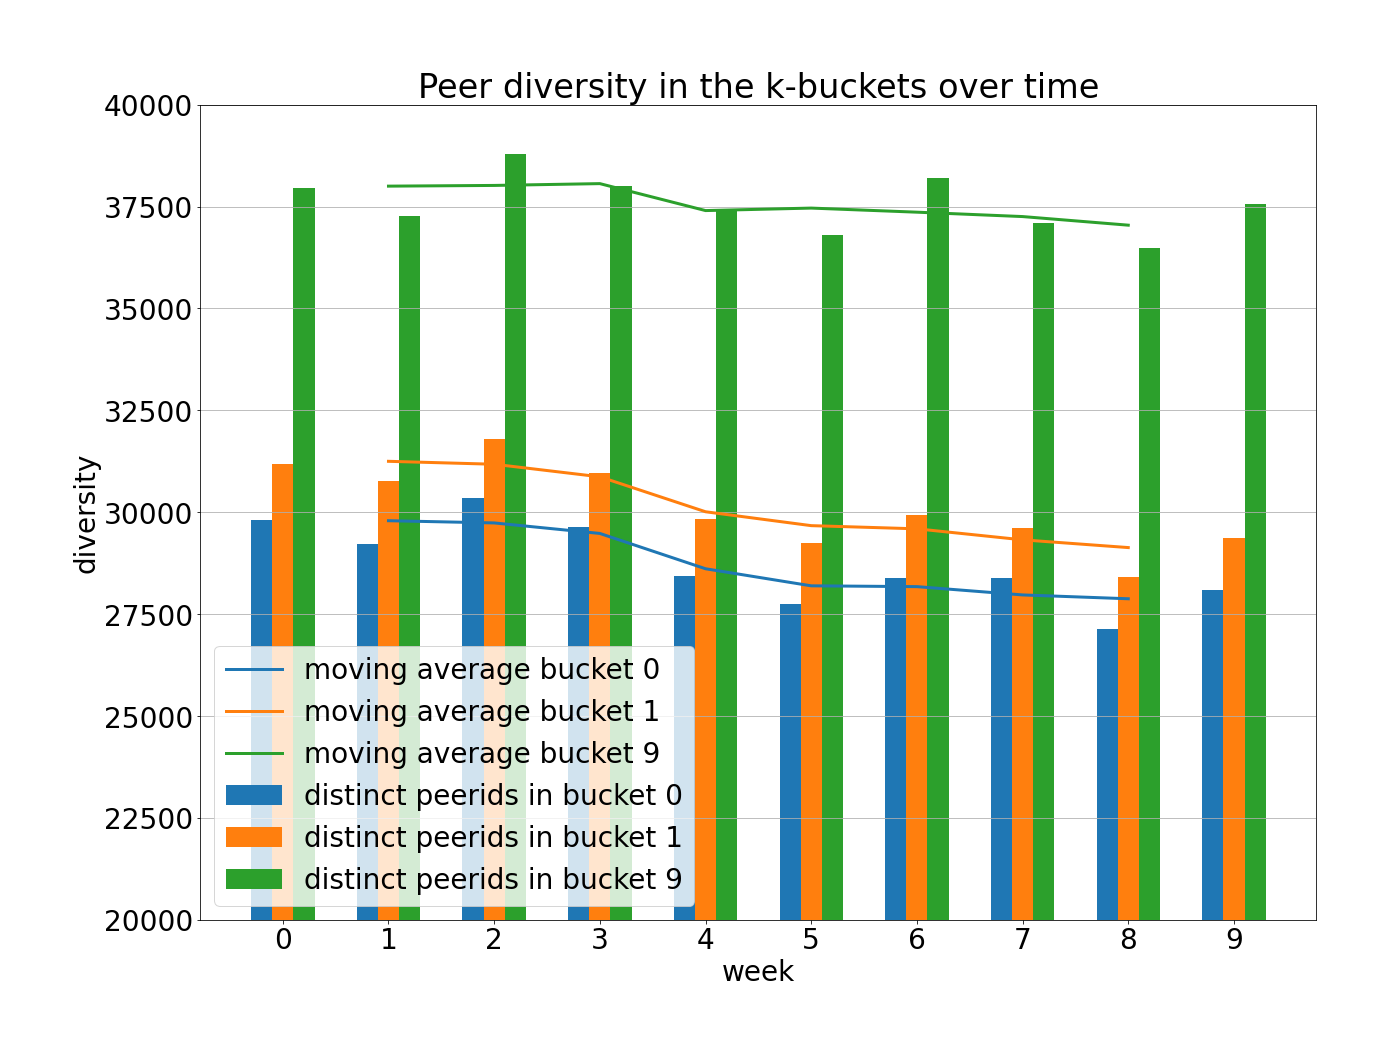
\includegraphics[width=\textwidth]{plots/diversity-b0-b1-b9.png}
    \end{center}
\end{column}
\end{columns}
\end{frame}

\fi

\begin{frame}
\frametitle{Conclusion}
\begin{itemize}
	\item Very low rate of stale entries in the routing table, given high churn
	\item Peers distributions in the \texttt{k-buckets} as expected
	\item the \texttt{k-buckets} are only missing a small number of peers
	\item \texttt{95.2\%} of the nodes have at least 18 of their 20 closest peers in their Routing Table
	\bigskip
	\item All results of \hyperlink{https://github.com/protocol/network-measurements/blob/rfm19/results/rfm19-dht-routing-table-health.md}{\texttt{RFM19}} of are available on the \hyperlink{https://github.com/protocol/network-measurements}{\texttt{protocol/network-measurements}} Github repo
	\item New measurements on diversity in the \texttt{k-buckets}! The DHT may become centralized over time. Make sure to attend the \texttt{Measuring IPFS} track at IPFS þing on Friday \texttt{2022-07-15} to learn more about it :)
\end{itemize}
\end{frame}

\begin{frame}
\frametitle{References}
\begin{enumerate}
	\item \hyperlink{https://github.com/protocol/network-measurements/blob/rfm19/results/rfm19-dht-routing-table-health.md}{\texttt{RFM19}} on the \hyperlink{https://github.com/protocol/network-measurements}{\texttt{protocol/network-measurements}} Github repo
	\item DHT Routing Table Health \hyperlink{https://www.notion.so/pl-strflt/DHT-Routing-Table-Health-f8e6836c4b09440baa909a4448a88fbf}{Notion page}
	\item \hyperlink{https://ipfs.io/ipfs/QmaVrnwZrnoG4YramcN75mbE5AUfCymiEErrHGXoQR968V}{Kademlia Paper} by Petar Maymounkov and David Mazières
	\item \hyperlink{https://github.com/dennis-tra/nebula-crawler}{Nebula Crawler} by Dennis Trautwein
	\item \hyperlink{https://github.com/guillaumemichel/py-binary-trie}{Python Binary Trie implementation}
	\item \hyperlink{https://www.notion.so/pl-strflt/ProbeLab-Protocol-Benchmarking-Optimization-a63238fd1b184d6f8fea4bb38d975208}{ProbeLab Notion page}
\end{enumerate}
\end{frame}



\end{document}